%%%%%%%%%%%%%%%%%%%%%%%%%%%%%%%%%%%%%%%%%%%%%%%%%%%%%%%%%%%%%%%%%%%%%%%%%%%%%
%	e-Yantra, IIT-Bombay

%	Document Author: keyur rakholiya
%					 Akshit gandhi
%	Date: 16-August,2012
%	Last Editted by: Saurav
%   Date Last updated: 31-05-2016 

%%%%%%%%%%%%%%%%%%%%%%%%%%%%%%%%%%%%%%%%%%%%%%%%%%%%%%%%%%%%%%%%%%%%%%%%%%%%%

\documentclass[11pt,a4paper]{article}
\usepackage{graphicx}
\usepackage{float}
\title{Calculations}
\author{keyur Rakholiya \\ Akshit Gandhi}
\date{\today}

\begin{document}
	\maketitle
	\newpage
	\tableofcontents
	\newpage
	\section{Tutorial Name}
		\textbf{Calculations for deciding the components to
		be used for drone(quadcopter)}

	\section{Theory and Description}
		First, calculate the approx weight of whole quadcopter\\
		1. Weight of frame = 300 gm\\
		2. Weight of bettary = 600 gm\\
		3. BLDC Motors = 4x85 gm\\
		4. Propellers = 4x15 gm\\
		5. Esc + R pi + FC(apm)= 200 gm\\
		6. Camara + gimble = 300 gm\\
		7. Buffer weight = 200 gm\\
		total weight = 2000 gm\\
		\\
		As per calculation,the total weight of drone is 2 kg about.
		So you need to generate 3 times of thrust of its weight for smooth lifting the quad and
		hovering.\\
		So we need to generate 6 kg of thrust from four motors.\\
		So each motor needs to generate 1.5 kg of thrust.\\
		Now according to required thrust we have to choose specified motors and propellers
		First of all, calculate the power.\\
		Equation for power is\\
		\\
		\begin{figure}[H]
			\centering
			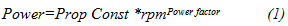
\includegraphics[width = 400 px]{equation1}
		\end{figure}
		
			\begin{figure}[H]
				\centering
				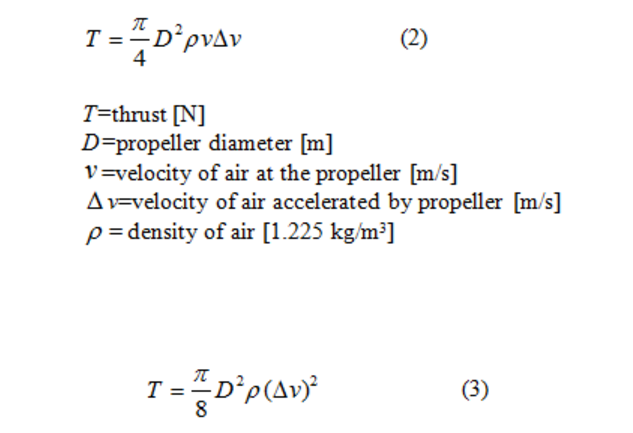
\includegraphics[width = 400 px]{eq2}
			\end{figure}
			
				\begin{figure}[H]
					\centering
					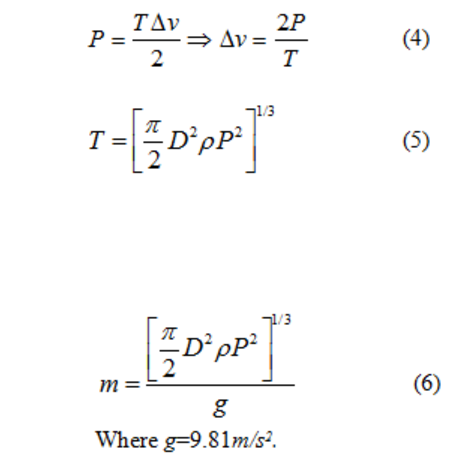
\includegraphics[width = 400 px]{eq3}
				\end{figure}
		Now calculate the power according to your propeller’s constant and put it in equation 6. it will give u thrust.
		Do the propeller test and get the readings, you can also find the prop test reading from
		sellers.
		
		choose your motors and propeller according to weight of your quadcoptr. follow the equations.
	\section{Experiment}
	we have choosen 1500 kva motors and 10x4E propellers.
		\begin{figure}[H]
			\centering
			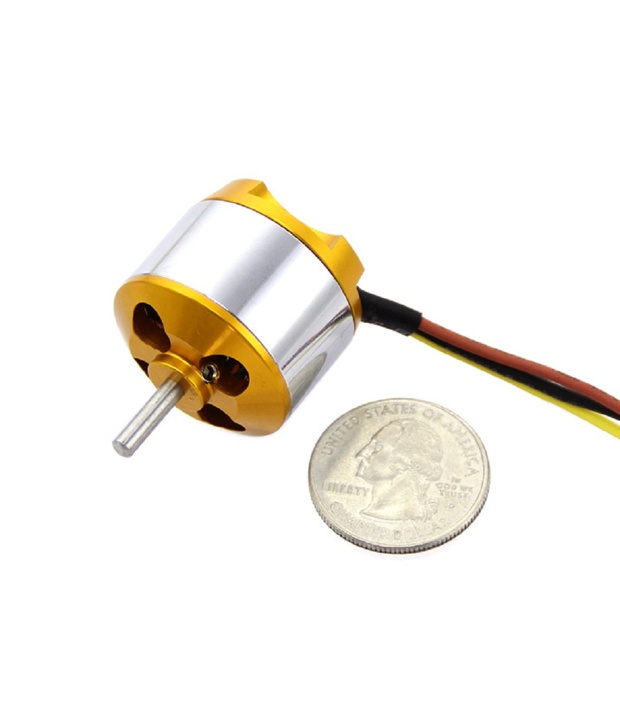
\includegraphics[width = 400 px]{mot}
			\caption{Brush less DC MOTOR 1500KVA}
		\end{figure}
		
		\begin{figure}[H]
			\centering
			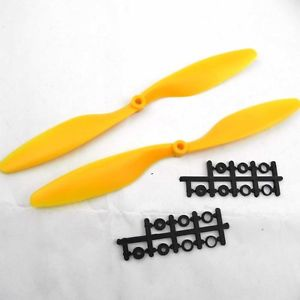
\includegraphics[width = 400 px]{prop}
			\caption{10x4E PROPELLER}
		\end{figure}
	\\
	\section{References }
	\url{https://quadcopterproject.wordpress.com/static-thrust-calculation/}
\end{document}



